% THIS IS SIGPROC-SP.TEX - VERSION 3.1
% WORKS WITH V3.2SP OF ACM_PROC_ARTICLE-SP.CLS
% APRIL 2009
%
% It is an example file showing how to use the 'acm_proc_article-sp.cls' V3.2SP
% LaTeX2e document class file for Conference Proceedings submissions.
% ----------------------------------------------------------------------------------------------------------------
% This .tex file (and associated .cls V3.2SP) *DOES NOT* produce:
%       1) The Permission Statement
%       2) The Conference (location) Info information
%       3) The Copyright Line with ACM data
%       4) Page numbering
% ---------------------------------------------------------------------------------------------------------------
% It is an example which *does* use the .bib file (from which the .bbl file
% is produced).
% REMEMBER HOWEVER: After having produced the .bbl file,
% and prior to final submission,
% you need to 'insert'  your .bbl file into your source .tex file so as to provide
% ONE 'self-contained' source file.
%
% Questions regarding SIGS should be sent to
% Adrienne Griscti ---> griscti@acm.org
%
% Questions/suggestions regarding the guidelines, .tex and .cls files, etc. to
% Gerald Murray ---> murray@hq.acm.org
%
% For tracking purposes - this is V3.1SP - APRIL 2009

\documentclass{acm_proc_article-sp}
\usepackage{listings} 
\usepackage{algorithmicx}
\begin{document}

\title{Schema-Aware Recommendation Engine for SQL Queries}

%
% You need the command \numberofauthors to handle the 'placement
% and alignment' of the authors beneath the title.
%
% For aesthetic reasons, we recommend 'three authors at a time'
% i.e. three 'name/affiliation blocks' be placed beneath the title.
%
% NOTE: You are NOT restricted in how many 'rows' of
% "name/affiliations" may appear. We just ask that you restrict
% the number of 'columns' to three.
%
% Because of the available 'opening page real-estate'
% we ask you to refrain from putting more than six authors
% (two rows with three columns) beneath the article title.
% More than six makes the first-page appear very cluttered indeed.
%
% Use the \alignauthor commands to handle the names
% and affiliations for an 'aesthetic maximum' of six authors.
% Add names, affiliations, addresses for
% the seventh etc. author(s) as the argument for the
% \additionalauthors command.
% These 'additional authors' will be output/set for you
% without further effort on your part as the last section in
% the body of your article BEFORE References or any Appendices.

\numberofauthors{2} %  in this sample file, there are a *total*
% of EIGHT authors. SIX appear on the 'first-page' (for formatting
% reasons) and the remaining two appear in the \additionalauthors section.
%
\author{
% You can go ahead and credit any number of authors here,
% e.g. one 'row of three' or two rows (consisting of one row of three
% and a second row of one, two or three).
%
% The command \alignauthor (no curly braces needed) should
% precede each author name, affiliation/snail-mail address and
% e-mail address. Additionally, tag each line of
% affiliation/address with \affaddr, and tag the
% e-mail address with \email.
%
% 1st. author
\alignauthor
Vishnu Pratish\\
       \affaddr{University of Waterloo}\\
       \affaddr{200 University Avenue West}\\
       \affaddr{Waterloo, Ontario, Canada}\\
       \email{vpratis@uwaterloo.ca}
% 2nd. author
\alignauthor
Pragnya Addala\\
       \affaddr{University of Waterloo}\\
       \affaddr{200 University Avenue West}\\
       \affaddr{Waterloo, Ontario, Canada}\\
       \email{paddala@uwaterloo.ca}
}
% There's nothing stopping you putting the seventh, eighth, etc.
% author on the opening page (as the 'third row') but we ask,
% for aesthetic reasons that you place these 'additional authors'
% in the \additional authors block, viz.
% Just remember to make sure that the TOTAL number of authors
% is the number that will appear on the first page PLUS the
% number that will appear in the \additionalauthors section.

\maketitle
\begin{abstract}
In this paper, we present a recommendation engine for SQL query language that can be used in the everyday life of a SQL query writer. We use a schema aware approach unlike our predecessors who use user history from query logs.  The key features of our recommendation engine are auto improvisation of attribute recommendations as the user types query and join predicate recommendation using statistical inference. We use a ranking system with weightages for various parameters at different contexts to recommend keywords, table names, column names and boolean conditions.

We evaluate the system using query logs on northwind database and has shown that we are able to recommend useful features 99\% of times in the top ten results and over 90% of times in the first two results.  
\end{abstract}

\terms{Recommendation}

\keywords{SQL, Recommendation System, autosuggestion, join predicate} % NOT required for Proceedings

\section{Introduction}
SQL is a universal language used by software engineers on a regular basis. Databases schemas are often designed by experts who are aware of the system and programmers often end up not having much familiarity with the schema. A software engineer who writes queries in a development environment based on this schema he will have to go back and forth to see the schema information to write effective queries. Doing this on a large scale system can be a tedious process. To explain this problem, we take the example of a user searching for the patient record of Englishman ``William Scott" in an hospital database. Schema complexity poses as the first challenge. Most hospitals have records of their patients in varied schema, typical to each department. Second, the user may not be fully aware of the exact values of the selection predicates, and may give only a misspelled or partial attribute value (in this case, the user knows him as ``Will"). Third, we would like the user to issue queries that are meaningful in terms of result size. A query listing all the patients in the hospital would not be helpful to the user, and in some cases could also be computationally expensive for the system. Lastly, we do not expect the user to be proficient in SQL to access the database. 

Structured query models like XQuery, and the wider known SQL are the current existing means provided by database systems to allow users to express complex query semantics. Though powerful, these query models are in essence difficult for users to adopt because they require users to fully understand the structure of the database (i.e., schema) and to express queries in terms of that particular structure. Most often, a developer due to inexperience, unfamiliarity with the database schema or mere lack of attention to computational complexity of the query, fails to use the optimal query. Recommendation engines for a SQL query have the potential to ease a programmer's life by providing him with possible suggestions and optimizations. Providing informed autosuggestions while writing the query can therefore ease a programmer's life.  We use an informed approach towards this end by using the information in hand like database schema, sample of data from the tables, already written partial query structure and semantic information on the schema. These information can be effectively used to give auto suggestions to the user who is writing the query. 

We present a simple recommender which makes the process of query writing easier.  Illustrating with an example, consider the following query and associated recommendations:

\lstset{language=SQL,breaklines=true}
\begin{lstlisting}[float=*]
SELECT --(suggest possible clauses to start the query)
Orders.OrderID, Customers.CustomerName --( No recommendations or as-you-type suggestions; incase of multiple column names, give preference to column within the same table) 
FROM Orders --(autofill table name based on suffix of select statement; incase of multiple table names, give preference to tables containing all the columns within itself over tables with join possibilities) 
INNER JOIN Customers --(suggest possible tables on which inner join could be done based on the data from Orders table) 
ON Orders.CustomerID=Customers.CustomerID --(suggest possible join predicate based on tables and column names); 
\end{lstlisting}

In this paper we discuss some observations which have helped us rank the suggestions, the implementation of the tool, and the tool`s evaluation using the standard Northwind database. We present a schema-aware recommendation system for SQL queries with a simple instant-response user interface. To evaluate the tool, we retrace the steps of some common queries used on Northwind database and evaluate the usefulness of the query recommendations given by the system.  

\section{Brief Survey}
We picked famous Northwind database schema and a couple of other database schemas and sample set of most frequently used queries on them, to arrive to the following inferences : 

1) In almost 90\% of ``join'' cases, column names are the same
\\2) In nearly 9\% of ``join'' cases, when column names are not same, column1 is a substring of column2 or vice versa.
\\3) In almost 99\% of ``join'' cases, datatypes of the matching column names are same with same length if VARCHAR is used. 

These inferences act as the key motivation for this work. 

\section{Implementation}
The key Data Strucutre that enables the reccomendations is a Global Index which acts as an in memory representation of schema on which various algorithms are applied to derive the reccomendations. Any relational database can populate this datastructure using a 'populateIndex()' interface exposed as an API.  

The base algorithm that that returns reccomendations is as follows : 

\begin {enumerate}
\item   User begins typing a partial SQL Query
\item  Parser suggests base keywords using a dictionary lookup of SQL keywords. A tokenizer converts the keywords into tokens. 
\item Tokens are serialized and passed into Global Index. 
\item Global Index , upon reciving the partial query, uses various algorithms to generate a list of reccomendations and join predicates(if necessary) based on the partial query and returns a ranked list of reccomendations. 
\item As user types in more information, substring matching is performed on this returend list of reccomendations and Step 3 is repeated (if required). 
\end {enumerate}


\subsection{Global Index Data Structure}
 A global index structure is populated which contains the schema information from database when a connect statement is detected. The implementation of this strucutre does not depend on the type of database used underneath. This is simply an object with sufficient methods and attributes to represent a schema and recommend on them. An overloaded `populateIndex()' method is written for each of the supported types of databases(currently only Mysql is supported) to populate this index. Hence adding support for new databases becomes relatively straightforward. 
The schema information essentially contains the table names, column names and datatype and key information for each of the tables. Apart from these a fraction of data is also collected from these 
Each database has its own way of extracting schema through the populate method. But the index structure just contains the information that is common to all relational databases in the market. Hence it simply becomes a matter of a few lines of code into the well defined interface of DBindex populateIndex() method to extend the feature to any databases.  

\subsection{Optimized Autosuggestions}
Most SQL editors of today provide user with simple suggestions but no ranking mechanism is involved. Our idea is to include ranking based on multiple criteria and return a ranked list of possible query snippets. This would help users decide which suggestion would be more relevant to them, besides providing the ease to users who are not fully familiar with the schema of the database that they are working on.

The suggested tool provides the user with the ten most relevant snippets, with an option to scroll down for more suggestions. The tool hugely makes use of the partial query entered and the database schema to predict/suggest rest of the query. This helps in narrowing down the list of reccomendations and improving the accuracy. Suggestions ranging from simple ones such as ``select'',``insert into'', ``update'', ``delete'' at the beginning of the query to more complex ones such as recommending possible join predicates are included. With ``select'' being the mostly commonly used SQL query it is given higher rank followed by the rest of the clauses. The tool has currently been built with more focus on the select statement as the scope for autosuggestions for this statement alone was relatively big. In future, we intend to extend the focus onto other SQL statements as well.

While typing in the column name in a query, when no partial text is entered, an entire list of column names is returned. First column is suggested depending on the partial text typed it. As seen in Fig. 1, the user's partial entry which in this case is ``P'' is used to suggest all the possible column names.  If the query involves two or more columns, columns within same table are given a static score of 50 and columns in other tables are given a score of 25. Succeeding columns are hence suggested using these scores thereby giving more preferences to columns within the same table over columns from different tables. Every insertion of comma in the query after a column name, brings out the possible ranked list of suggestion for remaining columns.

\begin{figure*}
\centering
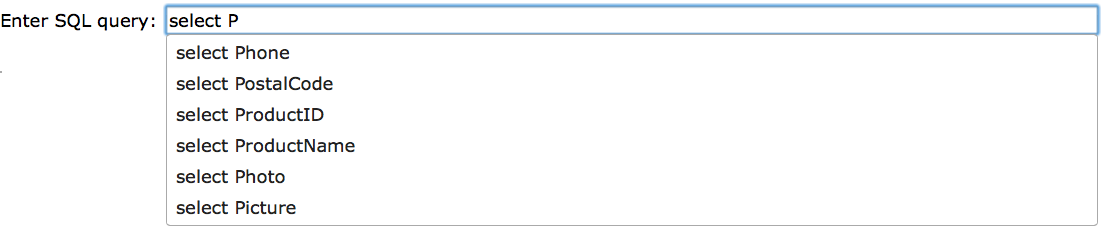
\includegraphics[width=170mm]{column_names}
\caption{Recommendations for Column Names}
\label{overflow}
\end{figure*}

SQL clauses such as ``from'', ``where'' etc. are suggested basing on the preceding part of the query, more specifically on the immediately preceding phrase.

Table names are determined by the column names used the earlier part of the query. Tables with all used column names within the same table are given a static score of 50 and tables with column names spanned across various tables are given a score of 25. As seen in Fig. 2, ``employees'' is ranked higher in the recommended list because the column names ``FirstName'' and ``Country'' are both present in ``employees'' table. The list is then followed by tables, `customers'' and ``suppliers'', which could be a part of the query incase of JOIN clause (basing on the column names). Like in the case of suggesting column names, usage of comma will bring out ranked suggestions for table names where tables with multiple column names within them are given higher preference over join possibilities.


\begin{figure*}
\centering
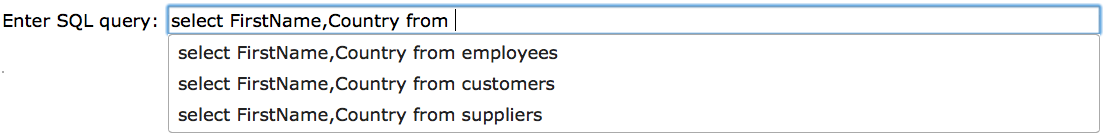
\includegraphics[width=170mm]{table_names.png}
\caption{Recommendations for Table Names}
\label{overflow}
\end{figure*}



\subsection{Join Predicate}
Join predicates form one of the key difficulties for every query writer. The complexity of possible ways in which a user can write join predicate translates to difficulty in creating a search space from which recommendations can be generated. To make the problem tractable, we treat join predicates as a separate entity with the following grammar:

\begin{verbatim}

<join_predicate> ::=
  <expression> [<outer_join_indicator>]
    <comp_op> <expression> [<outer_join_indicator>]

<outer_join_indicator> ::=
  (+) <!  This SQL clause is
          no longer recommended to be used
          and might be removed from future versions.  !>

<comp_op> ::=
  <
| >
| <>
| !=
| =
| <=
| >=
| ~= <!  for computers with ASCII code  !>
| ~< <!  for computers with ASCII code  !>
| ~> <!  for computers with ASCII code  !>

\end{verbatim}


The outer join indicator symbol is no longer recommended to be used and might be removed from future versions. Hence we ignored that operator. For a Join predicate of the form,  \textless expression\textgreater  \textless comp-op\textgreater \textless expression\textgreater, we followed a four step approach on generating recommendations. The data we already have include table names on which Join operation is being performed, and the column names to be used in the projection operator. These tokens are collected from the global parse structure  and passed to recommendation engine which in turn outputs the ranked join predicates. 

\subsubsection{Join Predicate prediction algorithm}
\begin {enumerate}
\item Find the Cartesian Product of columns on given tables with matching data type. This forms the search space from which recommendations are generated. Each recommendation is associated with a RecScore which decides the ranking of that particular recommendation. 
\item Columns with same column names are added a static score of 50.
\item Among the ones with same column name, columns with Primary Key  are added a score of 10.
\item Substring match one column name with another. If there is a full match, add 25 to the score. No score for partial matches 
\end{enumerate}

As seen in Fig. 4, columns with same name are listed at the top of the suggestion list of the join predicate, in this case - the top 5 recommendations. It is then followed by columns with substring matching, i.e. the next 2 recommendations. Datatype and character length matches come next on the list, recommendations 8 and 9. All the other possibilities are given lowest preference and can still be viewed by scrolling down the list.

\begin{figure*}
\centering
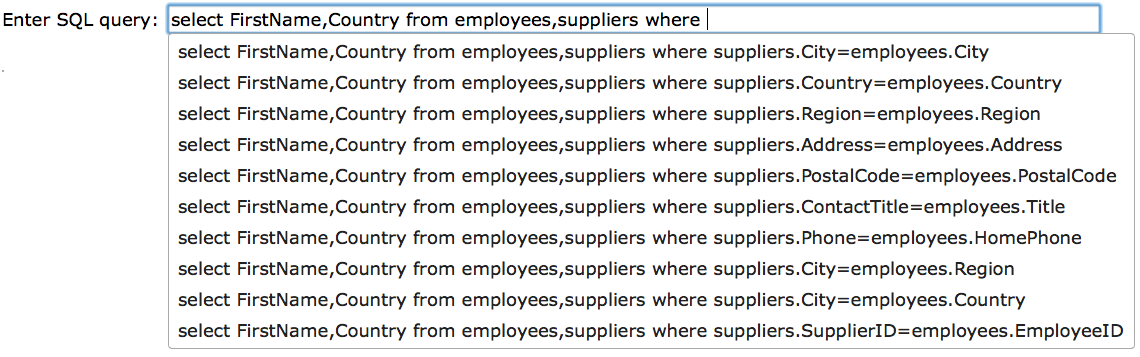
\includegraphics[width=170mm]{join_predicate.png}
\caption{Join Predicate sample recommendations}
\label{overflow}
\end{figure*}

\section{Evaluation}
We have taken a relatively straightforward approach to evaluate the efficiency of recommender. Evaluation is done for the fields which on which we are doing the prediction in the following manner. A database of queries on Northwind database was collected from various sources is used as test set. The same parser that was written to parse the partly written query for the reccomendation engine was used to construct an evaluator which basically compares between the recommendation suggested by our system and the one that is actually used in the query. 

\begin{figure*}
\centering
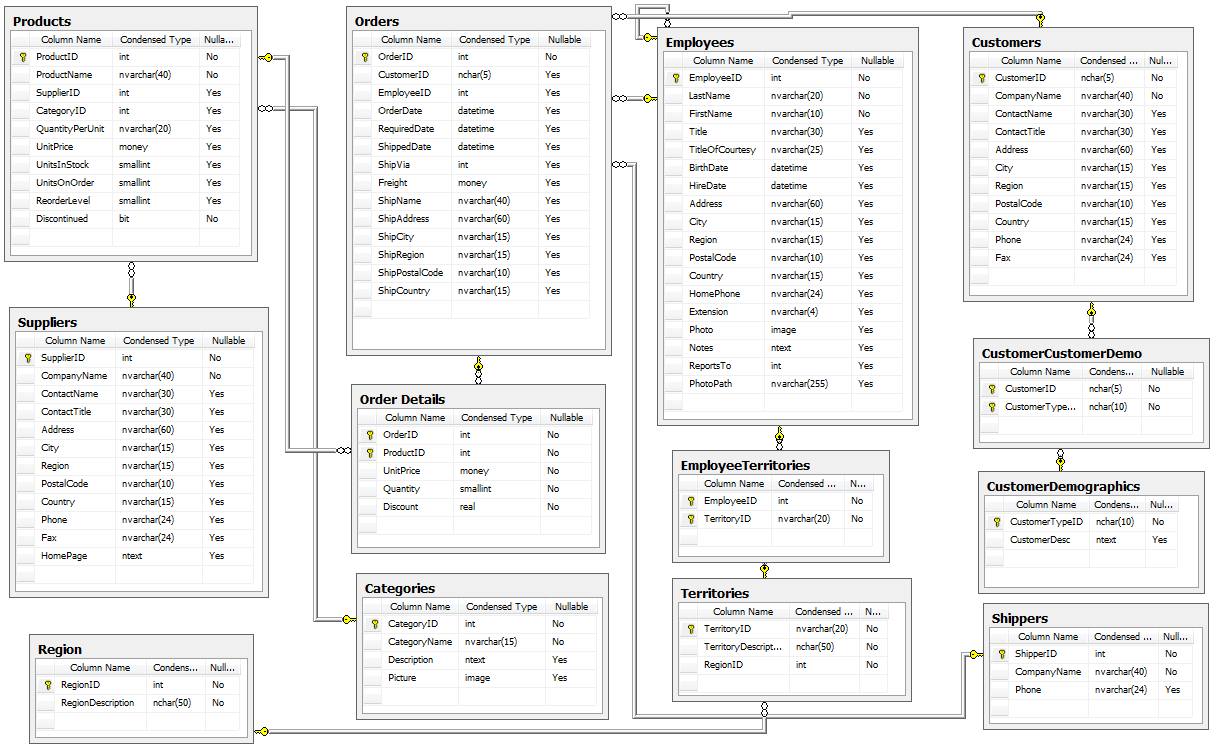
\includegraphics[width=170mm]{Northwind_schema.png}
\caption{Schema of NorthWind database}
\label{overflow}
\end{figure*}


There were 62 queries in our evaluation set collected from two different sources. With the features in our current recommendation system 65\% of the SELECT queries could be performed without errors. Other queries in the same set require nested joins, having or group by clauses etc. which would form a good part of future work. On retracing the do-able queries, in 86\% of the cases the recommendation at the top of the suggestion list matched the desired query. In 10\% of the cases the recommendation at the second or third spot in the suggestion list matched the desired query. Remaining 4% of suggestions was there in the top ten list as well. Hence, for the given sample set, we achieved 100\% accuracy in predicting the query, given the top 10 suggestions.

\section{Related Work}
Several tools and systems have been designed to ease the use of databases. Jagadish et al. [1] describe the most common challenges faced in databases today.

QueRIE [4], Javad Akbarnejad et al., was the one of the first frameworks to address the problem of generating SQL query recommendations. The QueRIE recommender system analyzes the query log of a user, searches for other users who have executed queries over similar parts of the database, and recommends new queries accordingly. 
Nodira Khoussainova et al. [5] present a system, SnipSuggest, to handle autocompletion for SQL queries basing on the context of the query.  It recommends possible additions to various clauses in the SQL query using related snippets collected from a log of past queries. 

Arnab Nandi et al. [2], discuss the issues of database schema and data complexity, result size estimation, and query validity; and provide novel approaches to solving these problems. Koutrika et al.[3] present a graph-based approach to automatically translate SQL into natural language and thereby provide the user with a textual explanation which would be helpful in common scenarios where the user is unaware of the semantic connections within various fields of a database. Extending SQL recommendation systems with such a feature would enrich their usability.

Many systems designed for databases mine old query logs. They focus on search logs of keywords[7, 8, 9], for tasks varying from predicting the next user action to designing a search taxonomy. Some others mine SQL query logs [10], to order the result tuples of a query. 

\section{Future Works}
\begin{itemize}
\item Semantic analysis \\
We have noted that the fieldnames that a schema designer uses to when the table is designed mostly falls into some standard names. These include dictionary words which conveys the meaning of the data contained within that attribute or appending suffixes like ``id'' or ``num'' or ``no'' to the attributes. This information has a potential of being used to provide better recommendations since we already have schema information in hand. For example, a semantic analysis of attributes would give information about the meaning of attributes which can be used to combine with already written partial query to provide similar recommendations.  

\item Integrating with IDEs\\
As of now this is simply implemented as a Javascript interface over a python 2.7 backend. The focus was on to develop the right algorithms for various SQL keywords. But for this to be used in the industry by a real software engineer, this has to be integrated with an IDE like Eclipse and an auto-connection detect feature needs to be implemented which can detect the connection statement and connect to existing databases prior to loading schema. 

\item Support for more databases through a uniform interface \\
The system now supports MySql which was used for test purposes. But the design is in such a way that it can easily be extended to support other databases with a few lines of code. 

\item Exploring the use case of SQL grammar\\
SQL grammar [insert reference here ] provides comprehensive information on the possible ways in which a SQL query can be constructed. This can be leveraged to provide recommendations on Keywords if not on attributes.  But more work is necessary to find how grammar can be incorporated into this. 

\item Nested joins, GROUP BY and HAVING clause\\
Support for Nested Joins, GROUP BY and HAVING clauses need further work in determinig how the generated reccomendation list can be ranked in an intutive manner. We are planning to include this in the next version. 

\end{itemize}

\section{Conclusion}
Enter text

\section{References}
[1] H. V. Jagadish, A. Chapman, A. Elkiss, M. Jayapandian, Y. Li, A. Nandi, and C. Yu. Making database systems usable. In Proc. SIGMOD, 2007.\newline
[2] A. Nandi and H. V. Jagadish. Assisted querying using instant-response interfaces. In Proc. SIGMOD, 2007.\newline
[3] G. Koutrika, A. Simitsis, and Y. Ioannidis. Explaining structured queries in natural language. In Proc. of the 26th ICDE Conf.\newline
[4] J. Akbarnejad, G. Chatzopoulou, M. Eirinaki, S. Koshy, S. Mittal, M. Eirinaki, Duc On and N. Polyzotis. SQL QueRIE Recommendations. In Proc. VLDB 2010.\newline
[5] Nodira Khoussainova , Yongchul Kwon , Magdalena Balazinska , and Dan Suciu. SnipSuggest: Context-Aware Autocompletion for SQL. In Proc. VLDB, 2010.\newline
[6] Georeference.org, Sample Queries.\newline
[7] A. Broder. A taxonomy of web search. SIGIR Forum, 2002.\newline
[8] D. Downey, S. T. Dumais, and E. Horvitz. Models of searching and browsing: Languages, studies, and application. In IJCAI, 2007. \newline
[9] D. Downey, S. Dumais, D. Liebling, and E. Horvitz. Understanding the relationship between searchers’ queries and information goals. In CIKM, 2008. \newline
[10] ] S. Chaudhuri, G. Das, V. Hristidis, and G. Weikum. Probabilistic ranking of database query results. In Proc. VLDB, 2004.



\end{document}
